\documentclass{article}
\usepackage{fontenc}
\usepackage[ngerman]{babel}
\usepackage[utf8]{inputenc}
\usepackage{graphicx}

\usepackage{datetime}
\newdateformat{myformat}{\THEDAY{ten }\monthname[\THEMONTH], \THEYEAR}

\begin{document}
	\begin{titlepage}
		\centering
		{\scshape\LARGE
			Ereignisdiskrete Systeme
			\par}
		\vspace{1.5cm}
		{\huge\bfseries Praktikum Blatt 1\par}
		\vspace{1.5cm}
		{\LARGE\itshape Jan Kristel, Alexandra Moritz\par}
		\vfill
			Aufsicht von Frau Rembold\par
			
		\vfill	
			{\large \today \par}	
		
	\end{titlepage}
	
	\tableofcontents
	\newpage
	\section{Aufgabe 1: MATLAB Grundlagen}
		\subsection{Was ist MATLAB?}
		\subsection{Wesentliche Komponenten der MATLAB-Oberfläche}
		\subsection{\textit{Current Folder Browser} - Wozu? Was ist zu beachten?}
		\subsection{\textit{Comand Window} - Was verbirgt sich dahinter?}
		\subsection{\textit{Tool-Strip} - Was verbirgt sich dahinter?}
		\subsection{Zweck des \textit{Workspaces}}
		\subsection{Möglichkeiten Information von \textit{MATLAB-Hilfe} zu bekommen}
		\subsection{Simulink}
		\subsection{\textit{Control System Tollbox} - Was ist das? Wo findet man sie?}
		\subsection{Stateflow}
		
	\newpage	
	\section{Aufgabe 2: Bodediagramme}
		\begin{figure}[h]
 		 	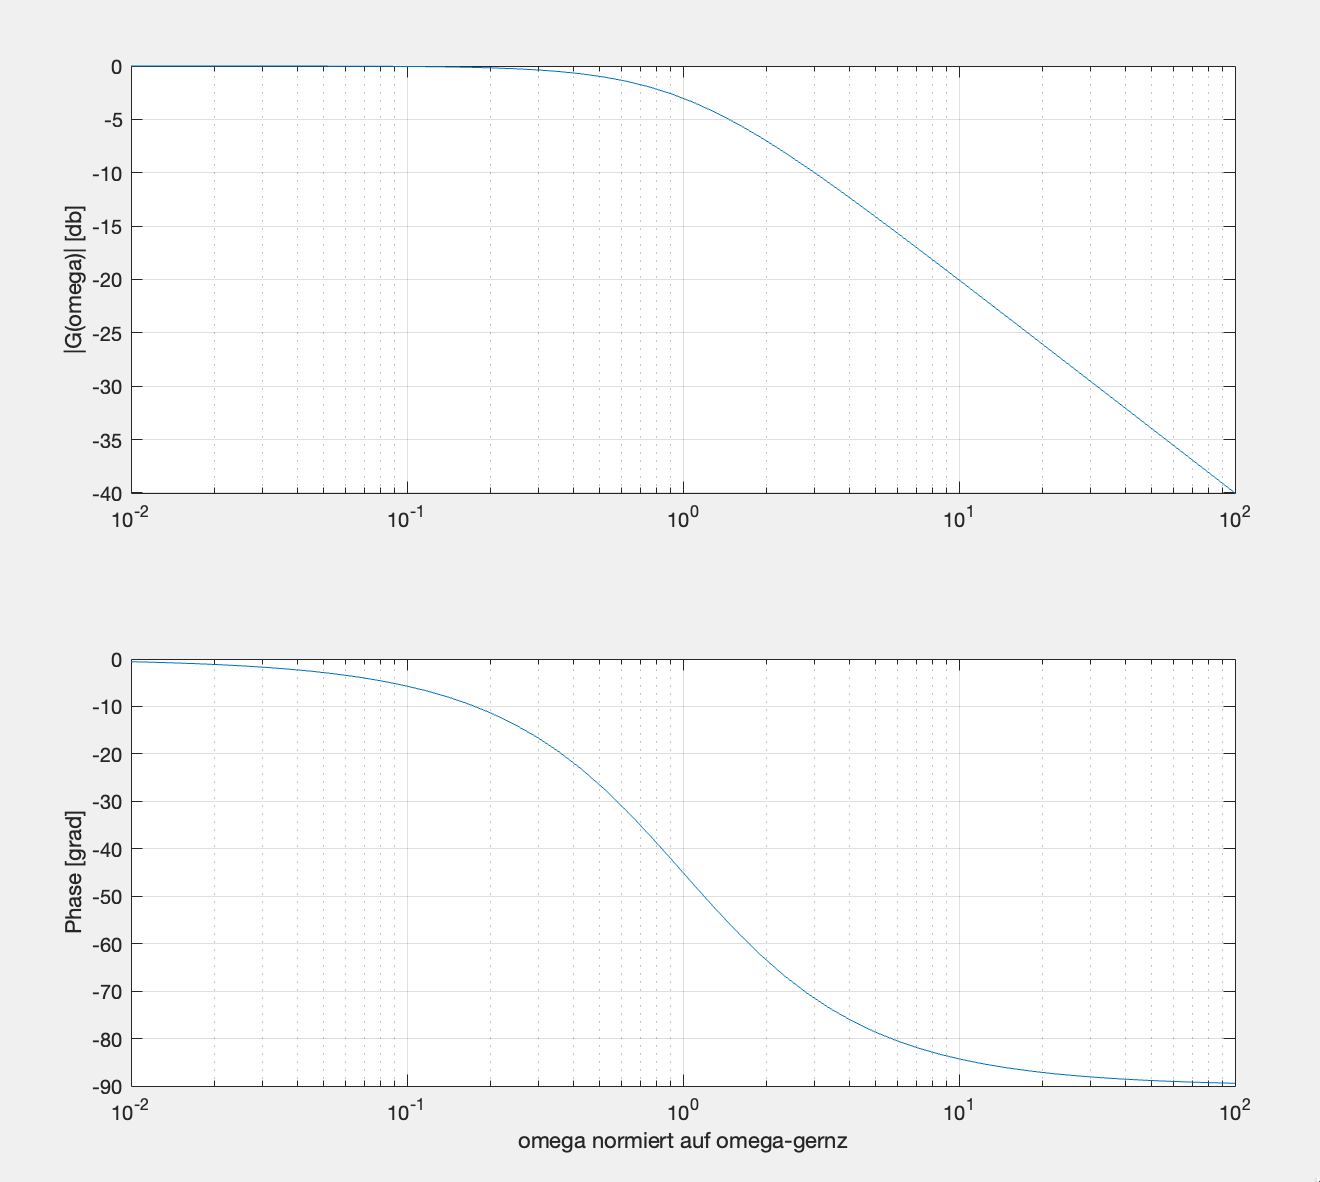
\includegraphics[scale=0.3]{Bodediagramme.png}
			\caption{Bodediagramme entstanden aus bodePT1.m}
			\label{fig1: Bodediagramm1}
		\end{figure}
		
		
		\subsection{Normierter Frequenzgang PT1-Glied}
		
		\subsection{Normierter Frequenzgang PT2-Glied}
	
	\newpage	
	\section{Aufgabe 3: Ortskurve}
	
	\newpage
	\section{Aufgabe 4: MATLAB Control System Toolbox}
	
\end{document}